\documentclass[12pt]{article}

\title{Linguistics 5 Notes}
\author{Andrew Tao}
\date{\today}

\usepackage{amsthm, lscape, tipa, tikz}

\newtheorem{dfn}{Definition}

\begin{document}

\maketitle

\section{Introduction}

Characteristics of Language

\begin{itemize}
\item[Semanticity] Specific signals, referred to as words, are tied to specific meanings
\item[Arbitrariness] There is no logical connection between the signal and its meaning
\item[Discreteness] Meaningful messages can be broken down into smaller, repeatable parts
\item[Displacement] Messages can refer to things outside of the current scope (time and space)
\item[Productivity] Users can understand and create never-before-head utterances
\item[Duality of Patterning] There is a pattern that governs the creation of larger meaningful messages from smaller discrete parts
\item[Cultural Transmission] Users must be exposed to the language to learn it (not inherent)
\item[Universal Grammar] Universal predisposition to expect vertain properties from language
\end{itemize}

\begin{dfn}[Grammar]
Grammar is a linguistic rule system that governs how we organize sounds, words, and sentences.
\end{dfn}

The structure of Linguistics

\begin{enumerate}
\item[Pragmatics] Study of how context contributes to meaning
\item[Semantics] Rules of how meaning is expressed
\item[Syntax] Rules of sentence formation
\item[Morphology] Rules of word formation
\item[Phonology] Rules of how sounds are combined
\item[Phonetics] The inventory of sounds available
\end{enumerate}

\begin{tabular}{r c c}
 & Descriptive Grammar & Prescriptive Grammar \\
 \cline{2-2} \cline{3-3}
Definition & Describes how language is actually used in everyday life & Describes how an authority defines the "proper" use of language \\
\end{tabular}

\begin{dfn}[Universal Grammar]
There is an inherent blueprint for grammatical rules shared across all humans and languages, referred to as universal grammar.
\end{dfn}

Noam Chomsky introduced the idea of generative grammar, the theory that there are a finite and precise set of rules capable to describe all possible sentences in a language.

\section{Phonetics}

\begin{dfn}[Phoneme]
A phoneme is the basic, distinctive unit of sound.
\end{dfn}

\pagebreak

\begin{landscape}
\subsection{Consonants}

\bigskip

\begin{tabular}{|p{1.1cm}|p{1.1cm}|p{1.1cm}|p{1.1cm}|p{1.1cm}|p{1.1cm}|p{1.1cm}|p{1.1cm}|p{1.1cm}|p{1.1cm}|p{1.1cm}|p{1.1cm}|p{1.1cm}|p{1.1cm}|p{1.1cm}|p{1.1cm}|}

\multicolumn{2}{|c|}{} & \multicolumn{2}{|c|}{Bilabial} & \multicolumn{2}{|c|}{Labiodental} & \multicolumn{2}{|c|}{Interdental} & \multicolumn{2}{|c|}{Alveolar} & \multicolumn{2}{|c|}{Palatal} & \multicolumn{2}{|c|}{Velar} & \multicolumn{2}{|c|}{Glottal} \\ \hline
\multicolumn{2}{|l|}{Stop} & p & b & & & & t & d & & k & g & & & & \\ \hline
\multicolumn{2}{|c|}{Fricative} & & & f & v & \textipa{T} & \textipa{D} & s & z & \v{s} & \v{z} & & & & \\ \hline
\multicolumn{2}{|c|}{Affricate} & & & & & & & & \v{c} & \v{j} & & & & & \\ \hline
\multicolumn{2}{|c|}{Nasal} & m & & & & & & n & & & & \textipa{N} & & & \\ \hline
\multicolumn{2}{|c|}{Glide} & m & w & & & & & l & & y & & & h & & \\ \hline
\multicolumn{2}{|c|}{Liquid} & & & & & & & r & & & & & & & \\ \hline

\end{tabular}
\end{landscape}

\subsection{Vowels}

\begin{tabular}{|c|}

\end{tabular}

Other miscelaneous features:
\begin{enumerate}
\item Diphthongs are two part vowel sounds.
\item Aspiration is a puff of air released after a consonant.
\end{enumerate}

Languages may also distinguish sounds through:
\begin{enumerate}
\item sound length
\item tone
\item stress
\item nasalization
\end{enumerate}

\section{Phonology}

Phonology is the study of the rules that govern our sound system.

Note that we can think of phonemes as the way we "think" about sounds, allophones as the way we actually "say" them.

\begin{dfn}
[Allophones] are predictable variants of a /phoneme/, where the distinction in question does not contribute to the meaning.

Minimal Pairs are pairs of words that share all the same characters but one and have different meanings.

\medskip

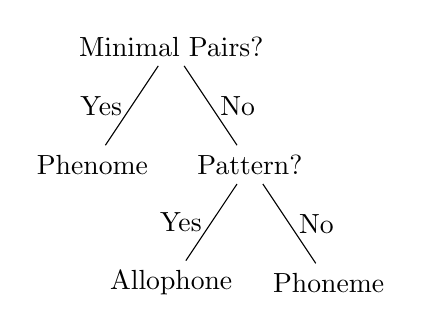
\begin{tikzpicture}
\node {Minimal Pairs?} [sibling distance = 2cm]
	child {node {Phenome} edge from parent node [left, black] {Yes}}
	child {node {Pattern?}
		child {node {Allophone} edge from parent node [left, black] {Yes}}
		child {node {Phoneme} edge from parent node [right, black] {No}}
	edge from parent node [right, black] {No}};
\end{tikzpicture}

\end{dfn}

Assimilation is the morphing of phonemes to be more similar to the phonemes around them. Dissimilation is when two neighboring sounds become less alike according to some feature.

Suprasegmentals look at parts of phonology bigger than a single sound. Ex: syllables, stress, intonation.

\section{Morphology}

Morpheme is the smallest unit of meaning in a language.

\subsection{Word Classes}

Parts of Speech / Syntactic Categories

\begin{itemize}

\item Content Words have concrete meanings we can easily define
\begin{itemize}
\item Noun
\item Verb
\item Adjective
\item Adverb
\end{itemize}
\item Function Words are defined according to their use/function
\begin{itemize}
\item Determiner (the, a, my, ...)
\item Numeral (one, five, ten, ...)
\item Quantifier (all, each, some, ...)
\item Pronoun (they, he, hers, ...)
\item Preposition (without, in , around, ...)
\item Conjunction (and, or, but, ...)
\item Degree Word (very, quote, so, ...)
\item Auxiliary Verb (have, be, do)
\item Modal (may, could, should, ...)
\end{itemize}
\end{itemize}

Free morphemes can stand by themselves, bound morphemes must be attached to something else. Roots form the basis of words.

Deriviational vs Inflectional Affixes. The former changes the type of word itself. The second gives more auxiliary changes (tense and the like).

Affixes:
\begin{itemize}
\item prefix
\item suffix
\item expletive infixation
\end{itemize}

\section{Morphological Typology}

Morphological typology is the study of the morphological similarities and differences across languages.

Analytic languages contain a lot more free morphemes/smaller words. Synthetic and polysynthetic languages contain words with more morphemes.

Fusion is when certain morphemes introduce more than one meaning to an affix.

Word formation processes
\begin{enumerate}
\item Compounding
\item Eponyms/Retronym
\item Blend
\item Conversion
\item Acronym
\item Clipping
\item Backformation
\item Reduplication
\end{enumerate}

\section{Syntax}

Syntax is the system of rules governing how words and constituents are arranged into larger constituents. We can find the syntactic category of a word from its position in a sentence.

English Grammar Rules

\begin{itemize}
\item[CL] NP Aux VP
\item[NP] (Det) (AP) N (XP)
\item[VP] V (XP)
\item[AP] (Deg) A
\item[AdvP] (Deg) Adv
\item[PP] (Deg) P (XP)
\item[Det] eg: that, some, the
\item[Aux] (modal) (have) (be) (do)
\item[Deg] eg: very, so, too
\end{itemize}

Ambiguity refers to the existence of multiple possible meanings.
\begin{itemize}
\item Lexical Ambiguity is when multiple word meanings are allowed
\item Syntactic Ambiguity is when sentence structures are allowed
\end{itemize}

Phrase Structure rule is a recursive rule.

Silent Syntax refers to parts of a sentence that are not physically there but affect the sentence. \\

Substitution is when we replace parts of a sentence with other parts. \\

Through parallelism, multiple same type clauses can be combined with coordination/conjunction words. \\

We take the base structure of a sentence, referred to as deep structure, then apply a series of movement rules to make a surface structure.

\section{Semantics}

Language follows a series of meaning rules. Sentences that break this are anomalous. \\

Lexical semantics provides us with more information on the conventions of word meanings. Semantic fields are subcategories based on semantic characteristics. \\

Words with related meanings are synonymous to polysemous. Words with opposing meanings are antonyms to homonyms. \\

There are semantic shifts in connotation and denotation through time. \\

Figurative language is deeply interconnected with semantics. There is still much intellectual discourse and research on all of this.

\subsection{Pragmatics}

Pragmatics is the study of meaning with context. This is the utterance meaning counterpart to literal meaning.

Sentences may be propositions that have a truth condition - they are either true or false regardless of context.

Analytic and synthetic sentences must be true from linguistic and real world facts. Contradictions are not true.

Speech Act explores meaning and actions. Utterances correspond to direct and indirect speech acts based on whether the intent is aligned with the utterance. These can be broken down into the following categories:
\begin{enumerate}
\item Interrogative: Question
\item Imperative: Command
\item Declarative: Statement
\end{enumerate}
Acts can be broken down into:
\begin{enumerate}
\item Locutionary: The literal meaning of the utterance
\item Illocutionary: The act performed by the utterance (inferences included)
\item Perlocutionary: The effect had on the audience
\end{enumerate}

Grice's maxims of cooperative conversation
\begin{enumerate}
\item Maxim of Quantity
\item Maxim of Quality
\item Maxim of Relevance
\item Maxim of Manner
\end{enumerate}

\end{document}